%%%%%%%%%%%%%%%%%%%%%%%%%%%%%%%%%%%%%%%%%%%%%%%%%%%%%%%
%                File: OpEx_temp.tex                  %
%                  Date: Sept. 2, 2009                %
%                                                     %
%           LaTeX template file for use with          %
%           OSA's journal Optics Express              %
%                                                     %
%  send comments to Jennifer Mayfield, jmayfi@osa.org %
%                                                     %
% This file requires style file, opex3.sty, under     %
%              the LaTeX article class                %
%                                                     %
%   \documentclass[10pt,letterpaper]{article}         %
%   \usepackage{opex3}                                %
%                                                     %
% Note that our online submission system does not     %
% currently process PDFLaTeX; if PDFLaTeX must be     %
% used, pls. contact OpEx staff, and we will process  %
% manually                                            %
%                                                     %
%                                                     %
%       (c) 2009 Optical Society of America           %
%%%%%%%%%%%%%%%%%%%%%%%%%%%%%%%%%%%%%%%%%%%%%%%%%%%%%%%

%%%%%%%%%%%%%%%%%%%%%%% preamble %%%%%%%%%%%%%%%%%%%%%%%%%%%
\documentclass[10pt,letterpaper]{article}
\usepackage{{../lib/opex3}}
%\usepackage{{../lib/penarandaY}}
\graphicspath{{../Pictures/}}
\usepackage{caption}
\usepackage{subcaption}
\usepackage{amsmath} % Required for equation and aligned environments
\usepackage{hyperref}
\RequirePackage{numprint}

%\usepackage{ae} %%for Computer Modern fonts

%%%%%%%%%%%%%%%%%%%%%%% begin %%%%%%%%%%%%%%%%%%%%%%%%%%%%%%
\begin{document}

%%%%%%%%%%%%%%%%%% title page information %%%%%%%%%%%%%%%%%%
\title{Chromatic Objective Optimization for Extended Depth of Focus \textit{(EDOF)}}

\author{M. Gostiaux Gabriel, M. Yohan Penaranda}

\address{M. Gabriel Gostiaux, Master of Science student, Institute of Optics, \\ Palaiseau, 91 120, France}

\email{gabriel.gostiaux@institutoptique.fr} %% email address is required

\address{M. Yohan Penaranda, Master of Science student, Institute of Optics, \\ Palaiseau, 91 120, France}

\email{yohan.penaranda@institutoptique.fr} %% email address is required

%\homepage{https://github.com/GabrielGst?tab=repositories} %% author's URL, if desired

%%%%%%%%%%%%%%%%%%% abstract and OCIS codes %%%%%%%%%%%%%%%%
%% [use \begin{abstract*}...\end{abstract*} if exempt from copyright]

\begin{abstract*}
This study introduces optimization through optical design softwares such as Zemax Optic Studio to basic concepts of co-design. The optimization can be monitored with matlab via the Zemax OS API, in order to optimize parameters of a chromatic imaging system dedicated to EDOF. In the end, the image will be post-processed using high-frequency transfer algorithm to enhance RGB image resolution.
\hfill \break

\textbf{Keywords:} EDOF, high frequency transfer, chromatic imaging system, Zemax OS API, Matlab.
\hfill \break

\end{abstract*}

%\ocis{(000.0000) General.} % REPLACE WITH CORRECT OCIS CODES FOR YOUR ARTICLE

%%%%%%%%%%%%%%%%%%%%%%% References %%%%%%%%%%%%%%%%%%%%%%%%%
\begin{thebibliography}{99}

%\bibitem{labwork} F. Goudail, D. Bloch, O. Leveque, ``FED labworks and projects,'' IOGS {\bf lab 3-4-5,} (2024)
\bibitem{trouve} P. TROUVE, ``Co-conception pourr la mesure 3D,'' IOGS, 11--25 (2024).
\bibitem{TNT+08} C.L. Tisse, H.P. Nguyen, R. Tessières, M. Pyanet, and F. Guichard. ``Extended
depth-of-field (EDoF) using sharpness transport across colour channels,'' In
Society of Photo-Optical Instrumentation Engineers (SPIE) Conference Series, {\bf volume 7061, page 4} (2008).

\end{thebibliography}

%%%%%%%%%%%%%%%%%%%%%%%%%%  body  %%%%%%%%%%%%%%%%%%%%%%%%%%
\section{Introduction}
One of the many objectives of co-design is to simulate optical designs in order to optimize costs through reducing the number of elements of the optical chain of a system. It is also possible to replace costly elements with hybrid ones, integrating signal and image processing in the system.

Here, we will focus on system modelling and optimization. In the first section we will see how using an optical design software helps with the modelling of such a chromatic system. We will see how optimizing the curvature radius and the focus, can be monitored by the criteria of maximizing the range within which at least one of the channels is resolved. Again, this is actually equivalent to maximizeing the union of the depth of focus of the three RGB channels of a chromatic camera within a range of interest. This generalized depth of focus (GDOF, \ref{eq:gdof}) will be computed in matlab through the Zemax OS API.  In the second section we will dive into the optimization of the chromatic system in the purpose of using it with the HFR algorithm. Thus, we will optimize it so that each channel have the best Modulation Transfer Function (MTF).

\begin{equation}\label{eq:gdof}
    G D O F=L \cap\left(\cup_{i \in R, V, B} D o F_i\right)
\end{equation}


\section{Co-Design of a Chromatic Imaging System with Zemax OS}
\subsection{Design simulation}

We work with the file \texttt{add-on-zemax.zmx} which provides a simple design, composed of an add-on and a paraxial lens. The add-on is composed of two different type of glass, separated by a spherical surface of radius $R$. It is this surface that will be optimized later on. The layout is presented on Fig. \ref{fig:layout}, and the chromatic aberration can already be seen to the experimented eye.

\begin{figure}[h]
	\centering
	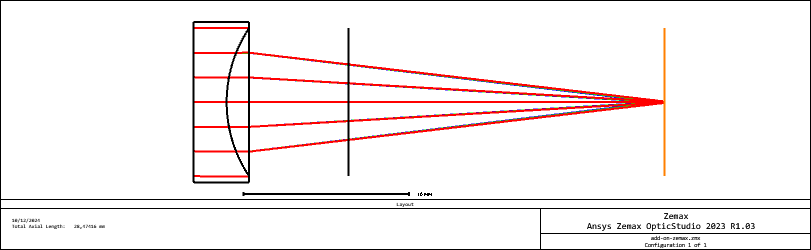
\includegraphics[scale=0.6]{Layout.png}
	\caption{System layout}
	\label{fig:layout}
\end{figure}

We present the analysis made with the tools provided by Zemax, the through focus spot diagram (TFSD) on Fig. \ref{sub@fig:through-focus} and the longitudinal aberration on Fig. \ref{sub@fig:lon-abe}. The TFSD is interesting because one can see the different focusing planes and the remaining RMS spot size of the other channels in those planes. On the longitudinal aberration, one can observe the focal shift of each channel when variating the field (y axis is the pupil coordinate).

\begin{figure}[h]
    \centering
    \subfloat[Through Focus Spot Diagram]{
        \centering
        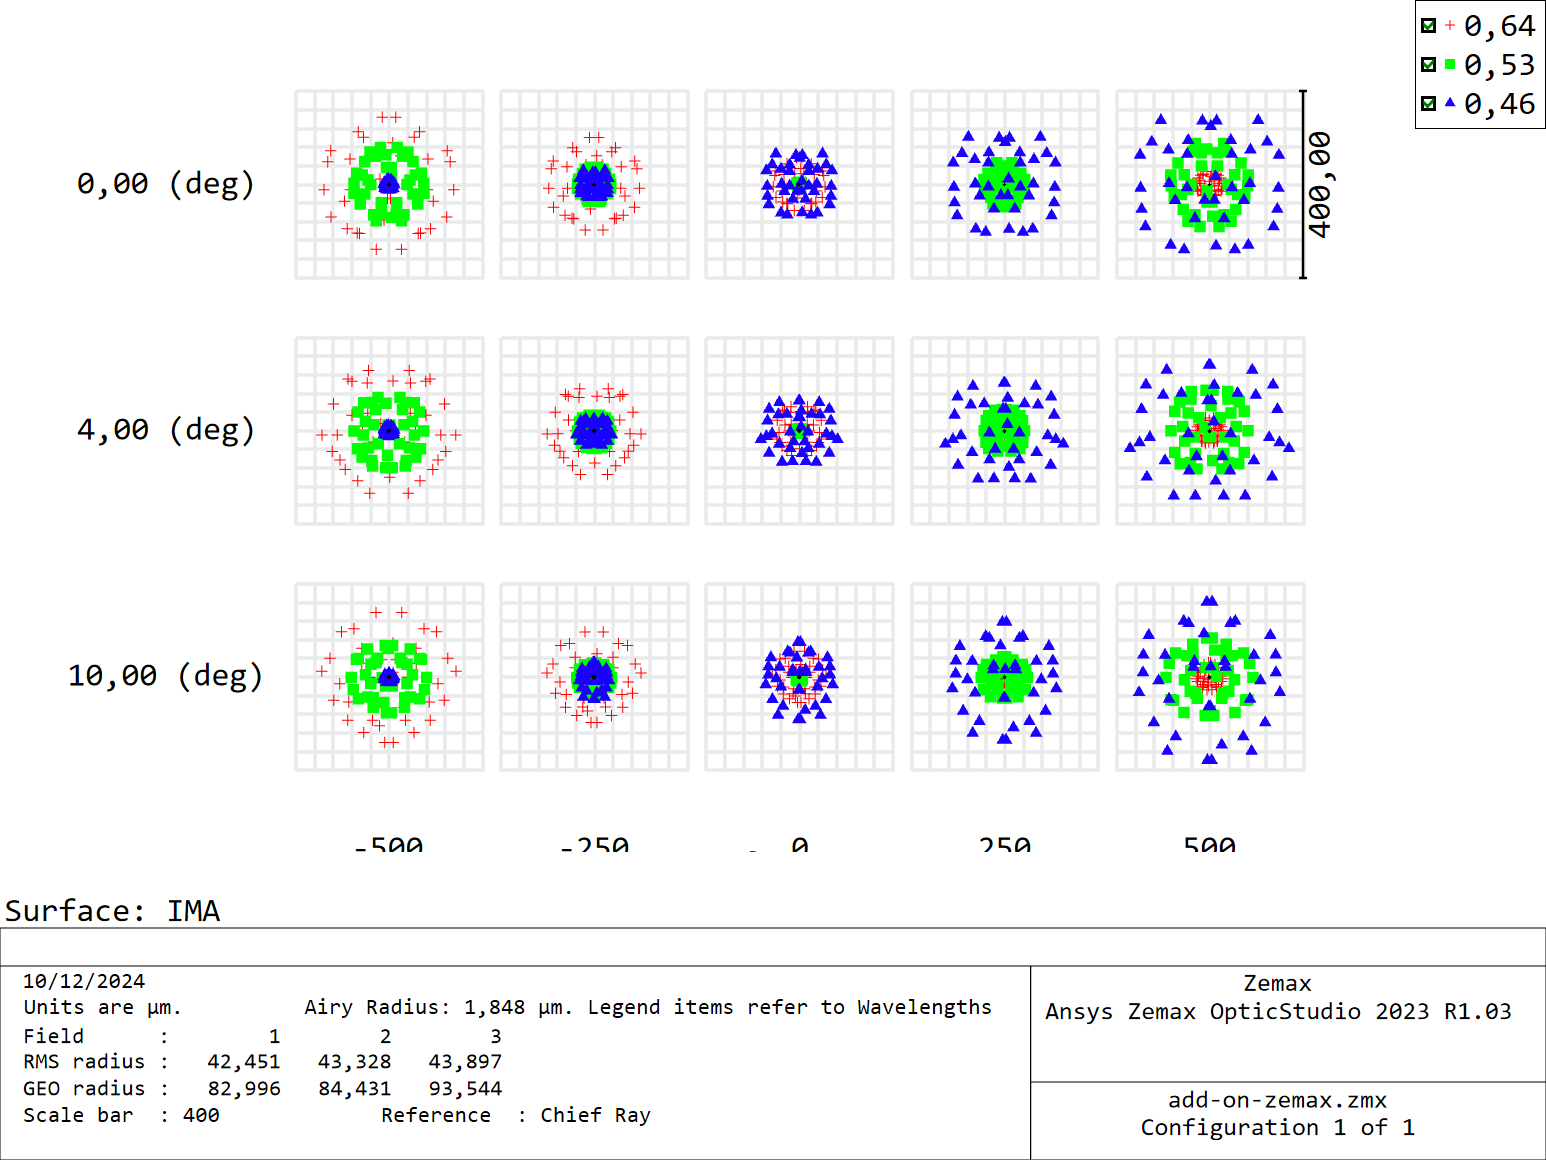
\includegraphics[width=0.4\textwidth]{ThroughFocusSpotDiagram.png}
        \label{fig:through-focus}
    }
	\subfloat[Longitudinal Aberration]{
		\centering
        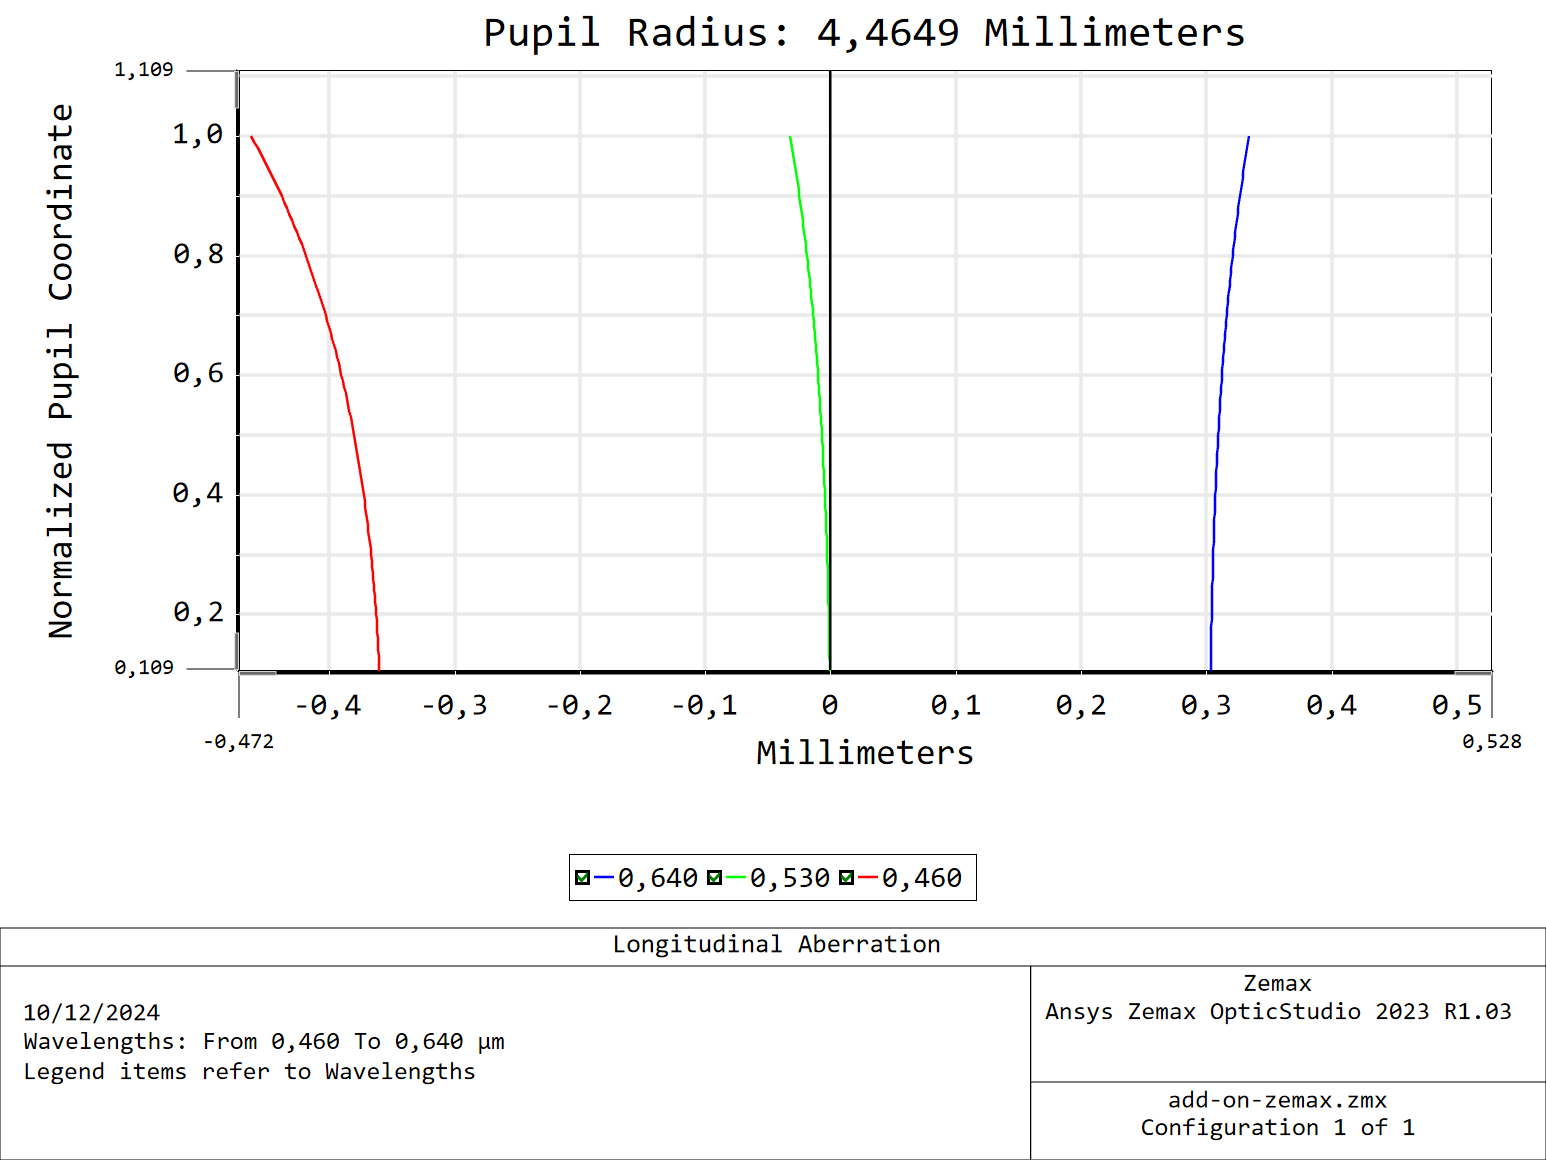
\includegraphics[width=0.4\textwidth]{LongitudinalAberration.png}
        \label{fig:lon-abe}
    }
	\caption{Chromatic aberration of the initial system}
\end{figure}

Thanks to these analysis, we can have a first estimation of the chromatic aberration: the longitudinal aberration is $\numprint[mm]{0.68}$ and this is confirmed by the longitudinal aberration diagram computed with Zemax, as can be seen on Fig. \ref{sub@fig:lon-abe}.
\begin{figure}[h]
    \centering
    \subfloat[MTF (Blue channel)]{
        \centering
        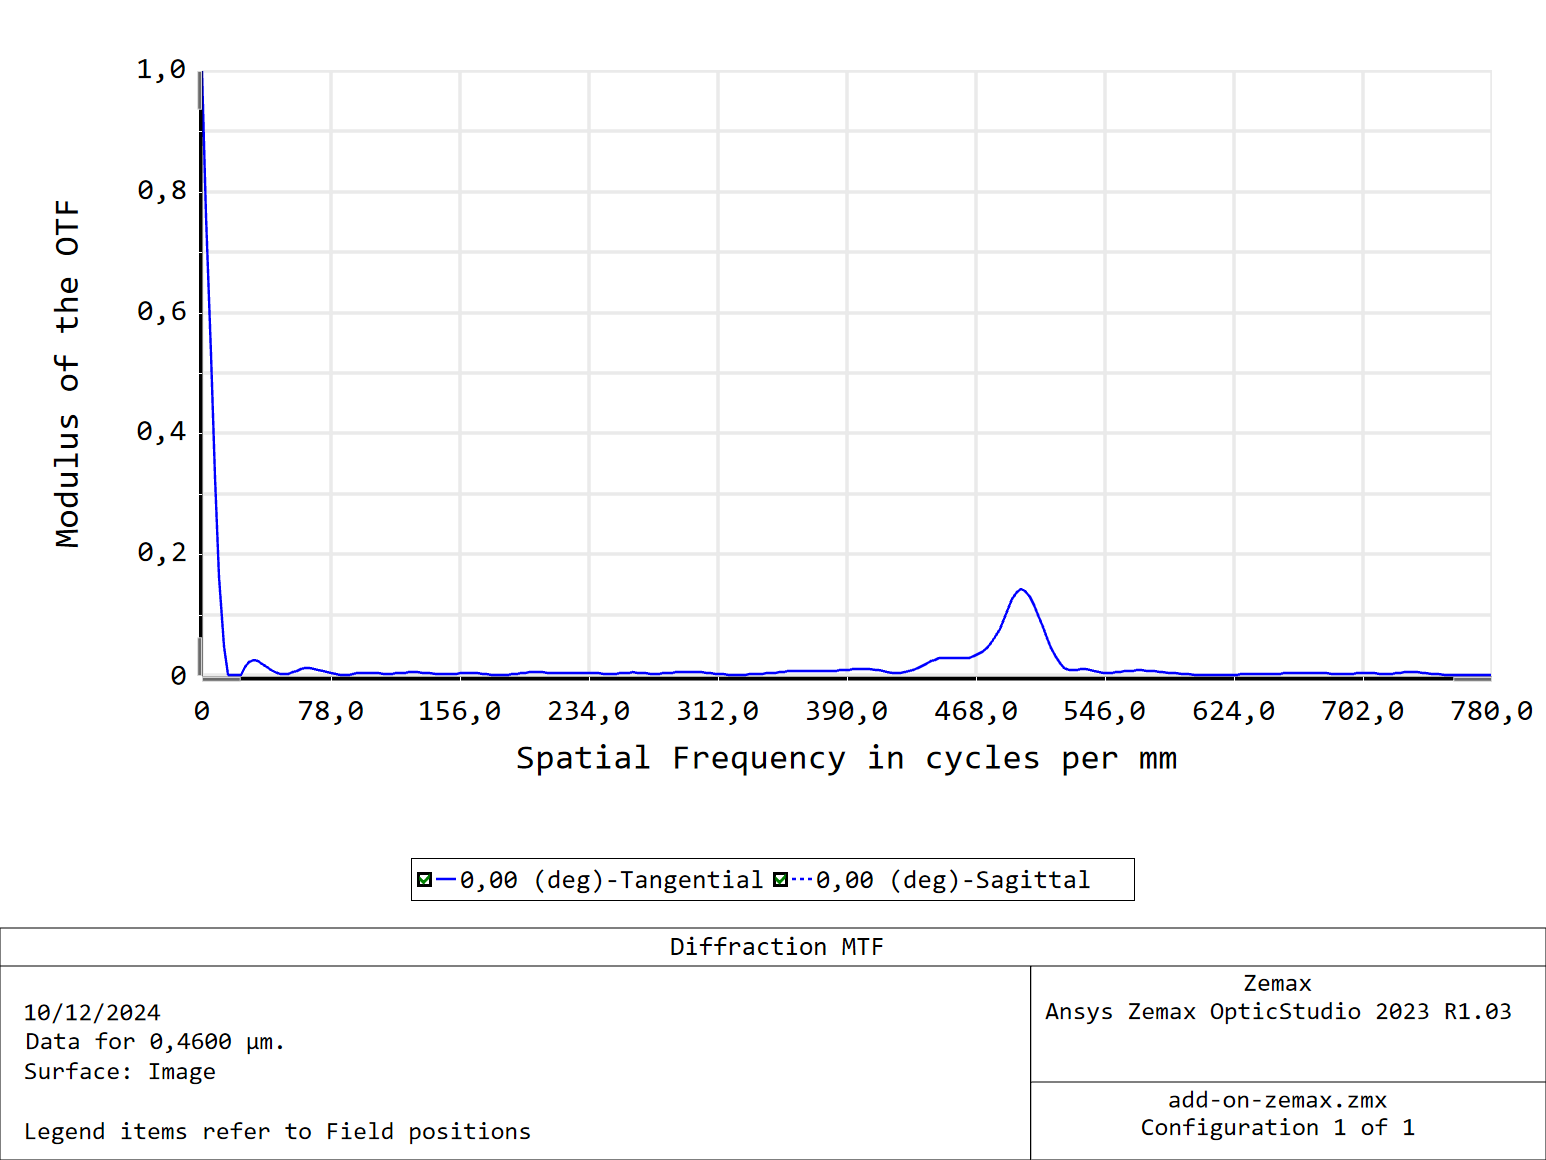
\includegraphics[width=0.3\textwidth]{FFTMTF_blue.png}
        \label{fig:fft-blue}
    }
	\subfloat[MTF (Green channel)]{
		\centering
        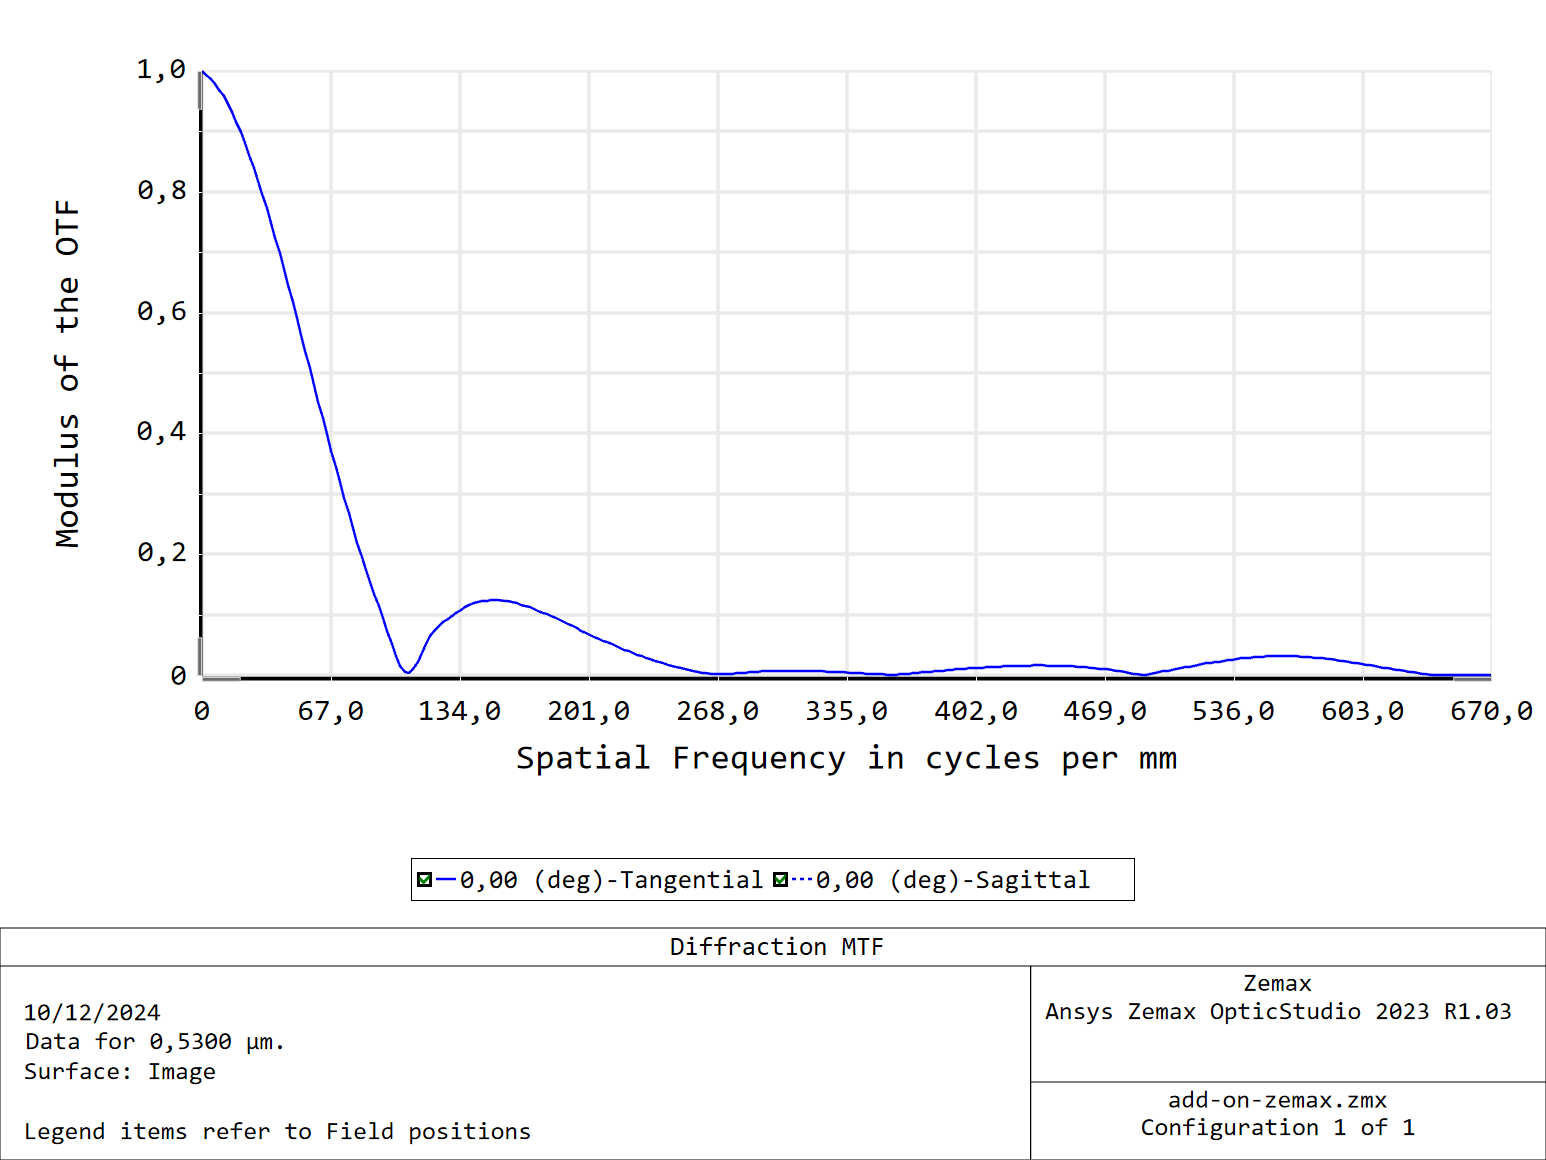
\includegraphics[width=0.3\textwidth]{FFTMTF_green.png}
        \label{fig:fft-green}
    }
    \subfloat[MTF (Red channel)]{
		\centering
        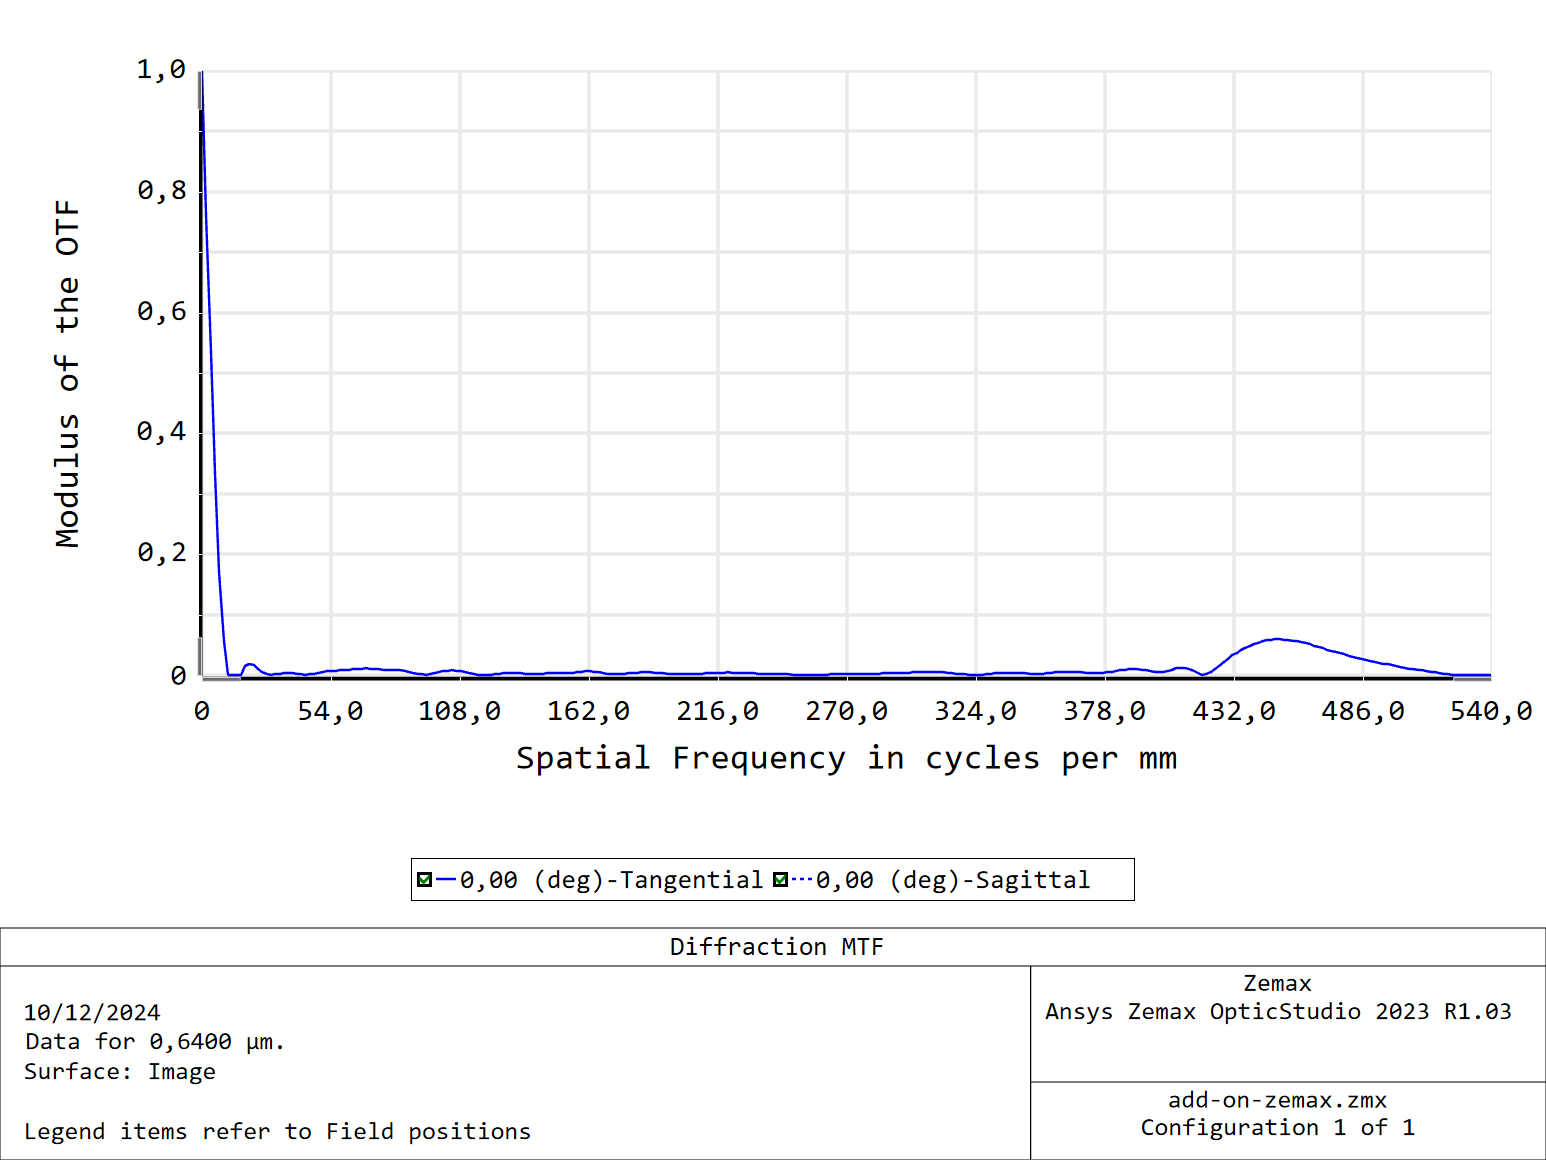
\includegraphics[width=0.3\textwidth]{FFTMTF_red.png}
        \label{fig:fft-red}
    }
	\caption{MTF of different channels}
    \label{fig:fft-colors}
\end{figure}

\paragraph{Initial configuration\\}
The sensor position considered in this study is $x'_0 = \numprint[mm]{19.160}$. The Spot Diagram figures allows the extraction of RMS values for different colors. At this position, the RMS radii for red, green, and blue channels are respectively $RMS_R = \numprint[\mu m]{42.210}$, $RMS_G = \numprint[\mu m]{3.063}$, and $RMS_B = \numprint[\mu m]{57.572}$. Indeed, the system optimizes the focal plane to match the focal plane of the green chanel, as it is the most sensitive for the human eye. The panchromatic ($RMS_{init} = \numprint[\mu m]{41.129}$) gives a rough idea of the overall performance of the system and is given in the spot diagram fig.\ref{fig:Spot_diag_init}.

\begin{figure}[h]
    \centering
    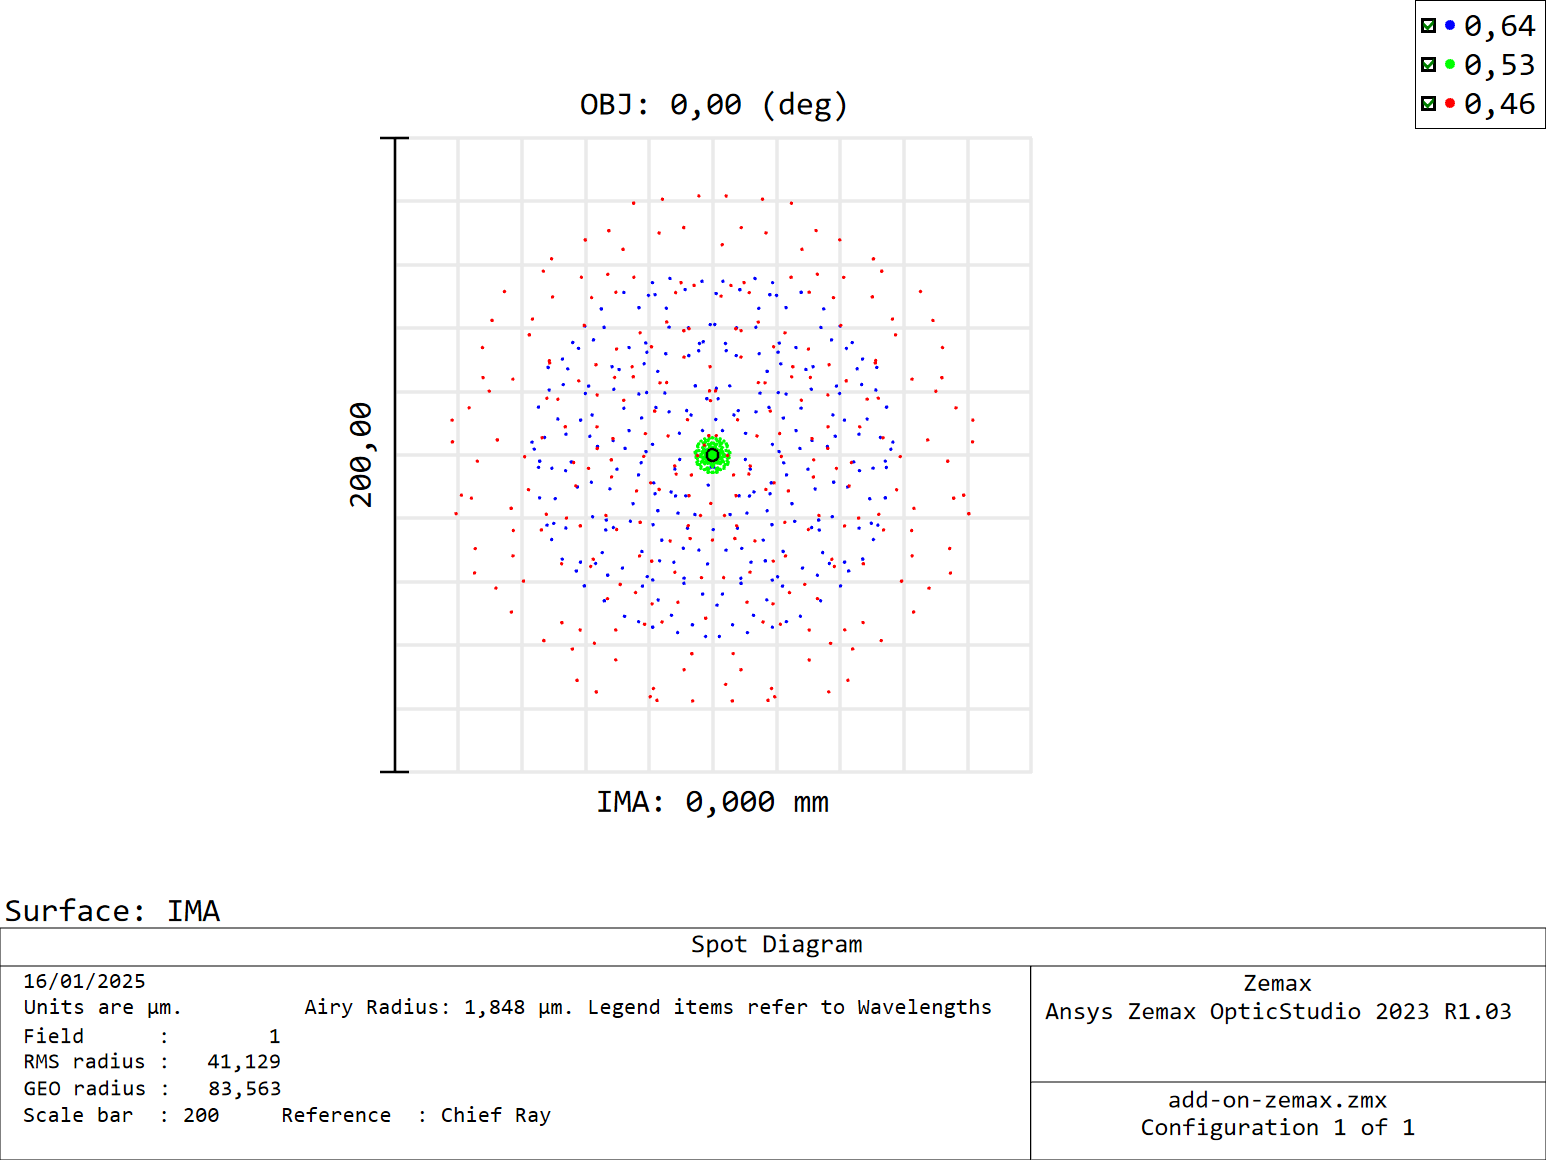
\includegraphics[width=0.8\textwidth]{IO25_TP4_SpotDiagram_init_2000.png}
    \caption{Spot diagram of the initial system.}
    \label{fig:Spot_diag_init}
\end{figure}

\paragraph{After quick focus\\} \label{manual-qf}
A quick focus (Optimize $>$ Manual Adjustment $>$ Quick Focus, option “Spot Size Radial” without “Use centroid”) is performed. The new sensor position is $x'_0 = \numprint[mm]{19.103}$. The new Spot Diagrams gives, for red, green, and blue, respectively $RMS_R = \numprint[\mu m]{48.827}$, $RMS_G = \numprint[\mu m]{3.991}$, and $RMS_B = \numprint[\mu m]{50.769}$. However, the overall RMS radius is relatively smaller, from $RMS_{init} = \numprint[\mu m]{41.129}$ to $RMS_{QF} = \numprint[\mu m]{40.633}$.



\subsection{GDOF computation driven through Matlab with ZOS API}

The function get\textunderscore RMS\textunderscore SpotSize.m was used to directly interface with an instance of Zemax from Matlab to extract the RMS Spot Size. 

This function was modified to retrieve this value for the three channels R, G, and B, for the system with a focus that minimizes the RMS spot size (Quick Focus). The results were obtained for a curvature radius corresponding to the one used in the Zemax file, which is $R= \numprint[mm]{8}$. 

A piece of the code used follows:

\begin{verbatim}
    % Value of the radius of curvature
    Surf_2.Radius=8;

    % We look at field 1
    spot_setting.Field.SetFieldNumber(1);

    % We set the object distance to 2 meters
    Surf_0.Thickness = 2000;

    % We perform a quick focus before retrieving RMS spot values
    QuickFocus = TheSystem.Tools.OpenQuickFocus();
    QuickFocus.RunAndWaitForCompletion();
    QuickFocus.Close();

    %...

    r0 = [r0, spot_results.SpotData.GetRMSSpotSizeFor(1,1)];
\end{verbatim}

Here, we first define the object to camera distance, then perform a quick focus and retrieve the RMS radii for the red, green, and blue channels. They were found to be $RMS_R = \numprint[\mu m]{41.623}$, $RMS_G = \numprint[\mu m]{4.089}$, and $RMS_B = \numprint[\mu m]{41.557}$, respectively. In the matlab file, the ray density is set to 6 with an hexapolar distribution, while the manual analysis have been performed with a ray density of 9 and dithered distribution, which explain the difference with paragraph \ref{manual-qf}. When the parameters are the same, the RMS are equal with matlab and manually. This shows that the RMS value depends strongly on the algorithm used and the parameters. Thus, every RMS are computed with the same parameters in the following.

\subsection{Performance criterion}
The performance criterion under optimisation is the Generalized Depth of Field (GDOF), which is defined as the range along the optical axis where the defocus remains below a threshold equivalent to the size of one pixel (5$\mu$m).

To evaluate the GDOF, we can utilize the RMS spot size, derived from the spot diagrams of geometrical ray tracing performed using the software. It serves as a metric for quantifying the spatial spread of rays at the image plane. A smaller RMS Spot Size corresponds to tighter convergence of rays, leading to reduced defocus and, consequently, an increased depth of field.
Following, a piece of code used:

\begin{verbatim}
    % We set the pixel pitch threshold
    dx = 25; %mm
    pp = 5.6; %µm
    
    threshold = pp * ones(size(object));

    % We compute the GDOF and display it
    R = result(2,:)<pp;
    V = result(3,:)<pp;
    B = result(4,:)<pp;
    gdof = (sum(R(:) == 1) + sum(V(:) == 1) + sum(B(:) == 1) ) * dx;
    disp(gdof)
\end{verbatim}

The computed value is $GDOF = \numprint[mm]{825}$ with quick focus performed for an object at $x_0 = \numprint[mm]{2000}$ and $R= \numprint[mm]{8}$. This value can be also see on fig.\ref{fig:gdof_init}. In this case, only the green chanel contributes to the GDOF.

\begin{figure}[h]
    \centering
    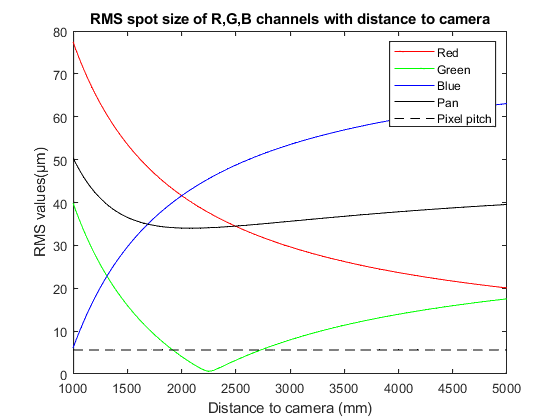
\includegraphics[width=0.8\textwidth]{IO25_TP4_GDOF_init_2000_R8.png}
    \caption{RMS radius of different colors depending on the distance of the object. The GDOF is the sum of the 3 independant depth of focus.}
    \label{fig:gdof_init}
\end{figure}

By modifying the radius of curvature of the surface, we are able to determine the best radius, giving the largest GDOF. The plot of GDOF according to the radius is shown fig.\ref{fig:gdof_opti}. We are aware that the curve does not correspond to the expactation. We did not manage to process the data that would gives the real representation. However, the actual value for the best radius is known to be $R_{opti}=\numprint[mm]{63}$, according to the analysis from past labworks.

With this new radius, the GDOF is at its maximum and the RMS spot size of each channels are displayed fig.\ref{fig:matlab_gdof}

\begin{figure}[h]
    \centering
    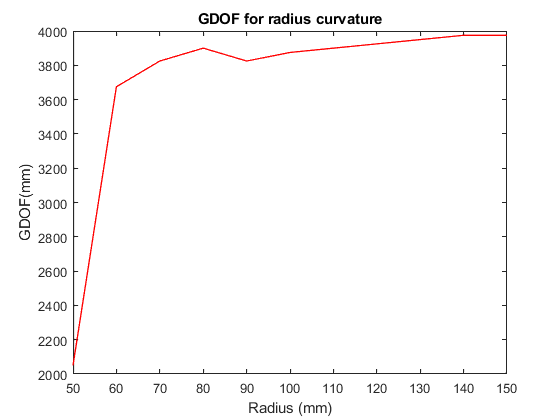
\includegraphics[width=0.8\textwidth]{IO25_TP4_optim_R_QF_2000.png}
    \caption{GDOF as a function of the radius. This curve should be interpreted with caution, as it does not accurately represent the real behavior. However, it has been included in the report as it is a result obtained through our experimental efforts.}
    \label{fig:gdof_opti}
\end{figure}

\begin{figure}[h]
    \centering
    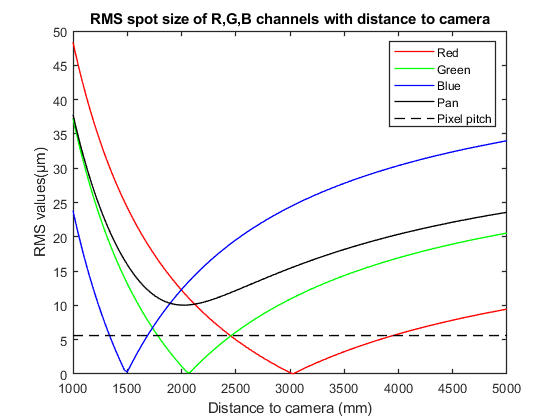
\includegraphics[width=0.8\textwidth]{matlab_gdof.png}
    \caption{RMS radius of each wavelenght depending on the distance of the object. With $R_{opti}=\numprint[mm]{63}$.}
    \label{fig:matlab_gdof}
\end{figure}

\section{Optimization for HFR post-processing}












\listoffigures

\end{document} 
